%%% CS6002 Project Report
%%% No-Regret Learning in Stackelberg Security Games with an Unknown, Bounded
%%% Set of Attacker Types.
%%%
%%% Written to emulate the AAMAS / ACM sigconf look without requiring acmart:
%%% two-column article, 9.5pt body, tight margins.

\documentclass[letterpaper,9pt,twocolumn]{extarticle}

\usepackage[top=0.85in,bottom=1in,left=0.75in,right=0.75in,columnsep=0.3in]{geometry}
\usepackage[utf8]{inputenc}
\usepackage[T1]{fontenc}
\usepackage{lmodern}
\usepackage{microtype}

\usepackage{amsmath,amssymb,amsthm}
\usepackage{mathtools}
\usepackage{bm}
\usepackage{enumitem}
\usepackage{graphicx}
\usepackage{booktabs}
\usepackage{algorithm}
\usepackage{algpseudocode}
\usepackage{xcolor}
\usepackage[hidelinks,breaklinks=true]{hyperref}
\usepackage[capitalise,noabbrev]{cleveref}
\usepackage{natbib}
\bibliographystyle{plainnat}

% ---- Balcan et al. notation ----
\newcommand{\pvec}{\mathbf{p}}
\newcommand{\svec}{\mathbf{s}}
\newcommand{\avec}{\mathbf{a}}
\newcommand{\cP}{\mathcal{P}}
\newcommand{\cE}{\mathcal{E}}
\newcommand{\cD}{\mathcal{D}}
\newcommand{\cC}{\mathcal{C}}
\newcommand{\cM}{\mathcal{M}}
\newcommand{\EE}{\mathbb{E}}
\newcommand{\NN}{\mathbb{N}}
\newcommand{\RR}{\mathbb{R}}
\newcommand{\Kmax}{K_{\max}}
\newcommand{\argmax}{\operatorname*{arg\,max}}
\newcommand{\argmin}{\operatorname*{arg\,min}}

% ---- Theorem / definition environments ----
\theoremstyle{plain}
\newtheorem{theorem}{Theorem}
\newtheorem{lemma}[theorem]{Lemma}
\newtheorem{proposition}[theorem]{Proposition}
\newtheorem{corollary}[theorem]{Corollary}
\theoremstyle{definition}
\newtheorem{definition}[theorem]{Definition}
\newtheorem{problem}[theorem]{Problem}
\theoremstyle{remark}
\newtheorem{remark}[theorem]{Remark}

% ---- Title block ----
\title{\vspace{-1.6em}\textbf{No-Regret Learning in Stackelberg Security Games\\
with an Unknown, Bounded Set of Attacker Types}\vspace{-0.2em}}
\author{\normalsize
Aditi Singh \qquad Ishita \qquad Sabil Ahmad\\
\footnotesize\textit{Indian Institute of Technology Bombay}\\
\footnotesize CS\,6002 Project, Spring 2026}
\date{\vspace{-1em}}

\begin{document}
\twocolumn[
  \begin{@twocolumnfalse}
  \maketitle
  \begin{abstract}
\noindent
In a \emph{repeated Stackelberg Security Game (SSG)}, a defender commits each
round to a randomized deployment of its resources and an adversarial sequence
of attackers, each drawn from some set $K$ of \emph{types}, best-responds.
\citet{balcan2015} designed no-regret online learning algorithms for this
model under the assumption that the set $K$ is \emph{known to the defender in
advance}, achieving expected regret $O(\sqrt{Tn^2 k\log(nk)})$ against an
oblivious adversarial sequence. They also show a matching lower bound:
linear-in-$T$ regret is unavoidable when $K$ is unrestricted. In practice,
however, the defender rarely knows $K$. We relax the known-$K$ assumption to
the natural middle ground $|K|\le\Kmax$, where the bound $\Kmax$ is known but
the actual types are discovered online. We propose \textsc{Grow-Catalogue}, an
algorithm that maintains the polytope partition of the coverage space
induced by the attacker types seen so far and re-runs an online learning
sub-routine whenever a new type is observed. We prove that under full-
information feedback \textsc{Grow-Catalogue} achieves expected regret
\[
 O\!\Bigl(\sqrt{T\cdot\Kmax\cdot\bigl(n^2+\Kmax\log n\bigr)}\Bigr),
\]
matching the bound of \citet{balcan2015} (with $k\mapsto\Kmax$) up to
constants. The bound is meaningful as long as $\Kmax\cdot(n^2+\Kmax\log n)\ll
T$; beyond this regime it is matched by the linear lower bound from the
unbounded side. We validate the theorem with experiments on synthetic SSG
instances under a staggered-uniform adversary, observing the predicted
sublinear behaviour and clear spikes in per-round regret at each discovery
round. Our implementation is available at
\textcolor{blue}{\href{https://github.com/CS6002-SSG/grow-catalogue}{github.com/CS6002-SSG/grow-catalogue}}.
  \end{abstract}
  \vspace{0.6em}
  \end{@twocolumnfalse}
]

% =============================================================================
\section{Introduction}
\label{sec:intro}

A \emph{Stackelberg Security Game} (SSG) models the strategic interaction
between a \emph{defender} protecting $n$ targets with limited resources and
an \emph{attacker} who chooses a target to attack. The defender commits to a
mixed strategy; the attacker observes the commitment and best-responds.
Computational tools built around this model are deployed at, among others,
the US Coast Guard, LAX airport, the Federal Air Marshals service, and
wildlife anti-poaching programs~\citep{tambe2012,yang2014}.

All such deployments require knowledge of the attacker's utility function.
In practice the defender faces many possible attacker types whose utilities
are only partially known. A natural online-learning formulation, due to
\citet{balcan2015}, treats the sequence of attackers as \emph{adversarial}:
at round $t$ an attacker of some type $a_t\in K$ arrives, and the defender
must maintain low regret against the best fixed commitment in hindsight.
\citet{balcan2015} show that for $|K|=k$ known and full-information feedback,
a polynomial-weights algorithm over the $\epsilon$-approximate extreme points
of the best-response polytope partition achieves expected regret
$O(\sqrt{Tn^2 k\log(nk)})$. They also prove that no online algorithm can
avoid $\Omega(T)$ regret in the fully unrestricted setting.

\paragraph{Motivation.}
The assumption that $K$ is known in advance is strong. A realistic
scenario is that the defender has domain knowledge of an \emph{upper
bound} $\Kmax$ on the number of distinct attacker types it might face
(e.g., ``at most five distinct threat actors''), but the utilities of any
particular attacker type are only revealed the first time that type
attacks. In this paper we ask:
\begin{center}
\emph{Can sublinear regret be achieved when the set of attacker types $K$
is unknown a priori but satisfies $|K|\le\Kmax$?}
\end{center}
This question sits cleanly in the gap between the ``known $K$'' setting and
the negative result for unrestricted $K$ in \citet{balcan2015}.

\paragraph{Contributions.}
Our contributions are as follows.
\begin{enumerate}[leftmargin=1.2em,itemsep=0.1em]
  \item \emph{Problem formulation.} We formalize the unknown-$K$ variant of
  the repeated Stackelberg security game (\Cref{sec:problem}).
  \item \emph{Algorithm.} We design \textsc{Grow-Catalogue}
  (\Cref{alg:gc}), which at each round maintains a catalogue $C_t$ of
  discovered attacker types, recomputes the set
  $\cE(C_t;\epsilon)$ of $\epsilon$-approximate extreme points of the
  partition of $\cP$ induced by $C_t$, and runs an anytime multiplicative-
  weights sub-routine over $\cE(C_t)$. When a new type is observed, the
  catalogue is updated and the sub-routine is restarted on the enlarged
  expert set.
  \item \emph{Regret bound.} We prove (\Cref{thm:main}) that
  \textsc{Grow-Catalogue} has expected regret
  $O(\sqrt{T\Kmax(n^2+\Kmax\log n)})$. This matches
  \citeauthor{balcan2015}'s Theorem~5.1 with $k$ replaced by $\Kmax$; for
  constant $\Kmax$ the rate is $\tilde O(n\sqrt T)$.
  \item \emph{Regime of applicability.} We characterize the range of
  $\Kmax$ for which the bound is non-trivial (\Cref{cor:regime}) and
  show that the instance-adaptive refinement depends on the number $K'$
  of types \emph{actually} observed, not on $\Kmax$.
  \item \emph{Experiments.} We implement \textsc{Grow-Catalogue} with
  two variants of the polytope recomputation (total and incremental) and
  evaluate them on synthetic SSG instances under a \emph{staggered-uniform}
  adversary. The measured regret is sublinear, with visible spikes at
  rounds of first appearance of each new type, confirming the epoch
  structure exploited by the proof (\Cref{sec:exp}).
\end{enumerate}

\paragraph{Organization.}
\Cref{sec:related} surveys related work. \Cref{sec:prelim} recalls the
Stackelberg security game formalism of \citet{balcan2015}. \Cref{sec:problem}
states the unknown-$K$ problem. \Cref{sec:analysis} presents the algorithm,
states the main regret theorem, and gives the complete proof.
\Cref{sec:exp} reports the experiments. \Cref{sec:conc} concludes.


% =============================================================================
\section{Related Work}
\label{sec:related}

The line of work most closely related to ours is online learning for SSGs
with \emph{attacker uncertainty}.

\paragraph{Prior-based approaches.}
\citet{pita2010} address uncertainty by solving a robust optimization problem
against worst-case attacker payoffs. \citet{kiekintveld2011} and
\citet{marecki2012} study \emph{Bayesian} SSGs in which a prior distribution
over attacker types is assumed; their algorithms require this prior, which
is usually estimated from historical data and hard to validate.

\paragraph{Learning a single unknown type.}
\citet{letchford2009} give a learning algorithm that, through best-response
queries, identifies the attacker's utility function with polynomial query
complexity. \citet{blum2014b} extend this to an ``adaptive commitment''
setting in which the defender refines its strategy round-by-round against a
single fixed, but unknown, type.

\paragraph{Adversarial sequence of types.}
\citet{balcan2015} depart from the single-type assumption. They model the
sequence of attackers as adversarially chosen from a \emph{known} finite set
$K$ and design no-regret algorithms for both full-information and partial-
information (bandit) feedback. Their full-information bound,
$O(\sqrt{Tn^2 k\log(nk)})$, is the starting point of our work. They also
prove an $\Omega(T)$ lower bound when $K$ is allowed to grow with $T$.

\paragraph{Online learning with changing expert sets.}
The internal sub-routine of \textsc{Grow-Catalogue} is an anytime variant of
the Polynomial Weights / Hedge algorithm
\citep{littlestone1994,freund1997,cesa2006}, which we restart each time the
catalogue changes. More sophisticated mechanisms for growing expert sets
exist \citep{mourtada2017,gaillard2019}; they shave logarithmic factors but
do not change the leading-order rate, and we stick with the simpler
restarting strategy.

\paragraph{Other related directions.}
\citet{haghtalab2022} study no-regret learning against non-myopic (strategic)
agents in a single-type query model. \citet{harris2024side} add \emph{side
information}: contexts observed by both players. Neither addresses the
``$K$ unknown but bounded'' question we pose here. To the best of our
knowledge no prior work combines the adversarial-types setting of
\citet{balcan2015} with an unknown $K$ of bounded size, although the gap
between \citeauthor{balcan2015}'s upper and lower bounds clearly invites this
extension.


% =============================================================================
\section{Preliminaries}
\label{sec:prelim}

We recall the formal model of \citet[\S 2]{balcan2015}, adopting their
notation throughout.

\paragraph{Game primitives.}
A repeated SSG has a time horizon $T\in\NN$, a set of targets
$N=\{1,\dots,n\}$, a defender with $R$ resources, and a collection
$\cD\subseteq 2^N$ of \emph{schedules}, each of which represents a set of
targets a single resource can defend simultaneously. An
\emph{assignment function} $A:R\to 2^{\cD}$ indicates the set of schedules
each resource may be assigned to. A \emph{pure strategy} is any valid
resource-to-schedule assignment. Let $m$ denote the number of pure
strategies, and let $M$ be the $\{0,1\}$-valued $n\times m$ indicator
matrix with $M_{i,j}=1$ iff target $i$ is covered under the $j$-th pure
strategy. A \emph{mixed strategy} is a distribution $\svec\in\Delta_m$ and
its induced \emph{coverage probability vector} is $\pvec=M\svec\in[0,1]^n$,
where $p_i$ is the probability that target $i$ is defended. The set
$\cP\subseteq[0,1]^n$ of valid coverage probability vectors is a convex
polytope.

\paragraph{Payoffs.}
Each target $i$ carries defender utilities $u_d^c(i)$ (if $i$ is attacked
and covered) and $u_d^u(i)$ (attacked and uncovered), both in $[-1,1]$. The
defender's \emph{expected} utility when target $i$ is attacked under
coverage $\pvec$ is
\[
U_d(i,\pvec)\;=\;u_d^c(i)\,p_i+u_d^u(i)\,(1-p_i),
\]
which is linear in $\pvec$ for fixed $i$.

\paragraph{Attacker types.}
An attacker \emph{type} $\alpha$ is a pair of utility vectors
$u_\alpha^c,u_\alpha^u\in[-1,1]^n$; its expected utility from attacking
target $i$ under coverage $\pvec$ is
$U_\alpha(i,\pvec)=u_\alpha^c(i)p_i+u_\alpha^u(i)(1-p_i)$. Observing
$\pvec$, type $\alpha$ \emph{best-responds} by attacking
\begin{equation}
b_\alpha(\pvec)\;=\;\argmax_{i\in N}\,U_\alpha(i,\pvec),
\label{eq:br}
\end{equation}
with ties broken arbitrarily but consistently.

\paragraph{Repeated game and regret.}
There is a (possibly unknown) set $K$ of attacker types. An
\emph{oblivious} adversary fixes a sequence
$\avec=a_1,\dots,a_T\in K^T$ before the game starts. At each round $t$ the
defender commits $\pvec_t\in\cP$, attacker $a_t$ best-responds, and the
defender receives $U_d(b_{a_t}(\pvec_t),\pvec_t)$. The defender's benchmark
is the best fixed coverage vector in hindsight,
\begin{equation}
\pvec^*\;=\;\argmax_{\pvec\in\cP}\;\sum_{t=1}^T U_d\bigl(b_{a_t}(\pvec),\pvec\bigr),
\label{eq:pstar}
\end{equation}
and the (expected) regret of an online algorithm is
\begin{equation}
\mathrm{Regret}(T)\;=\;\sum_{t=1}^T\! U_d\bigl(b_{a_t}(\pvec^*),\pvec^*\bigr)\!-\!\EE\!\Bigl[\sum_{t=1}^T\! U_d\bigl(b_{a_t}(\pvec_t),\pvec_t\bigr)\Bigr].
\label{eq:regret}
\end{equation}

\paragraph{Polytope structure.}
The following two lemmas of \citet{balcan2015} are the technical machinery
we will inherit. For a set of types $C\subseteq K$, a type $\alpha\in C$ and
a target $i\in N$, define
\begin{equation}
\cP_i^\alpha(C)\;=\;\bigl\{\pvec\in\cP\,:\,b_\alpha(\pvec)=i\bigr\},
\label{eq:Pi}
\end{equation}
a convex polytope defined by the pairwise linear inequalities
$U_\alpha(i,\pvec)\ge U_\alpha(j,\pvec)$ for all $j\ne i$. For a response
profile $\sigma:C\to N$ let
$\cP_\sigma(C)=\bigcap_{\alpha\in C}\cP_{\sigma(\alpha)}^\alpha(C)$;
the non-empty $\cP_\sigma(C)$ partition $\cP$ into convex regions in
which every $\alpha\in C$ has a fixed best response. Within each region the
defender's payoff as a function of $\pvec$ is \emph{linear}.

\begin{lemma}[\citealp{balcan2015}, Lem.\,4.3]\label{lem:43}
Fix $\epsilon>0$. There exists a finite set
$\cE(C;\epsilon)\subseteq\cP$ (the \emph{$\epsilon$-approximate extreme
points} of the partition induced by $C$) such that for any sequence
$\avec'$ of attackers from $C$ of length $T'$,
\[
\max_{\pvec\in\cE(C;\epsilon)}\!\sum_{t=1}^{T'}\!U_d(b_{a'_t}(\pvec),\pvec)\ge\max_{\pvec\in\cP}\!\sum_{t=1}^{T'}\!U_d(b_{a'_t}(\pvec),\pvec)-2\epsilon T'.
\]
\end{lemma}

\begin{lemma}[\citealp{balcan2015}, Lem.\,4.4]\label{lem:44}
The set $\cE(C;\epsilon)$ of \Cref{lem:43} can be chosen so that
$
 |\cE(C;\epsilon)|\in O\!\bigl((2^n+|C|n^2)^n\cdot n^{|C|}\bigr).
$
\end{lemma}

\begin{proposition}[\citealp{balcan2015}, Prop.\,1]\label{prop:hedge}
For any fixed expert set $\cM$ and any loss sequence in $[-\kappa,\kappa]$,
there is an online learning algorithm whose expected regret after
$T'$ rounds is at most $O\!\bigl(\sqrt{T'\kappa\log|\cM|}\bigr)$, without
requiring $T'$ to be known in advance.
\end{proposition}

\Cref{prop:hedge} is achieved, e.g., by Polynomial Weights / Hedge with a
time-varying learning rate $\eta_t=\sqrt{\log|\cM|/t}$, which gives an
\emph{anytime} guarantee; see \citet[\S 2]{cesa2006}.

% =============================================================================
\section{Unknown $K$ with a Known Bound $\Kmax$}
\label{sec:problem}

We depart from \citet{balcan2015} in exactly one point: the set $K$ is not
revealed to the defender at the start.

\begin{problem}[Unknown-$K$ repeated SSG]\label{prob:unknown}
A repeated SSG as in \Cref{sec:prelim} is played, with the following two
changes.
\begin{enumerate}[leftmargin=1.2em,itemsep=0.0em]
  \item The set $K$ of attacker types is \emph{unknown} to the defender at
  the start, but $|K|\le\Kmax$ for a known constant $\Kmax$.
  \item Feedback is \emph{full information}: at the end of round $t$ the
  defender observes $a_t$, and the first time any type $\alpha$ is
  observed, its utility vectors $(u_\alpha^c,u_\alpha^u)$ are revealed.
\end{enumerate}
The defender's benchmark and regret are still those of
\Cref{eq:pstar,eq:regret}.
\end{problem}

\begin{remark}[Necessity of a bound on $|K|$]
\citet[Thm.\,7.1]{balcan2015} show that if $|K|<2^{T+1}$ is unrestricted,
every online algorithm has regret $\Omega(T)$. Hence \emph{some} bound on
$|K|$ is needed for a sublinear guarantee; our assumption of a known
constant $\Kmax$ is the least restrictive such bound.
\end{remark}

\begin{remark}[Benchmark is well-defined]
The benchmark $\pvec^*$ of \Cref{eq:pstar} depends only on the realized
sequence $\avec$, which contains at most $\Kmax$ distinct types. So even
though $K$ is unknown to the defender, $\pvec^*$ itself is always a single
fixed element of $\cP$.
\end{remark}


% =============================================================================
\section{Algorithm and Analysis}
\label{sec:analysis}

\subsection{The \textsc{Grow-Catalogue} Algorithm}

At any round $t$, the defender holds a \emph{catalogue}
$C_t\subseteq K$ of types observed so far and the associated expert set
$\cE_t=\cE(C_t;\epsilon)$, where $\epsilon=1/\sqrt T$. An anytime
Polynomial-Weights instance is run over $\cE_t$. When a new attacker type
is observed, $C_t$ is enlarged, $\cE_t$ is recomputed, and the sub-routine
is restarted on the new expert set. \Cref{alg:gc} gives the pseudocode.

\begin{algorithm}[H]
\caption{\textsc{Grow-Catalogue} (full information)}
\label{alg:gc}
\begin{algorithmic}[1]
\small
\Require Horizon $T$; bound $\Kmax$; game primitives; default coverage
$\pvec_{\text{def}}$ (e.g.\ uniform)
\State $C\gets\emptyset$,~$\cE\gets\emptyset$,~$\epsilon\gets 1/\sqrt T$,~$t_{\text{loc}}\gets 0$
\For{$t=1,\dots,T$}
  \If{$\cE=\emptyset$}
    \State play $\pvec_t\gets\pvec_{\text{def}}$
  \Else
    \State sample $\pvec_t\sim q_t$ from the current PW distribution over $\cE$
  \EndIf
  \State observe $a_t$
  \If{$a_t\notin C$}\Comment{new type discovered}
    \State $C\gets C\cup\{a_t\}$; record $(u_{a_t}^c,u_{a_t}^u)$
    \State $\cE\gets\cE(C;\epsilon)$\Comment{recompute partition}
    \State restart PW on $\cE$; $t_{\text{loc}}\gets 0$
  \Else\Comment{routine update}
    \State $t_{\text{loc}}\gets t_{\text{loc}}+1$
    \State $\ell_t(\pvec)\gets -U_d(b_{a_t}(\pvec),\pvec)$ for each $\pvec\in\cE$
    \State $\eta\gets\sqrt{\log|\cE|/t_{\text{loc}}}$
    \State $w_{\pvec}\gets w_{\pvec}\,e^{-\eta\,\ell_t(\pvec)}$ for each $\pvec\in\cE$
  \EndIf
\EndFor
\end{algorithmic}
\end{algorithm}

We implement two variants of line 11: (i) \emph{total recomputation}, which
rebuilds $\cE(C;\epsilon)$ from scratch, and (ii) \emph{incremental}, which
reuses PW weights for extreme points that survive the new refinement of the
partition. The two variants are observationally equivalent -- they achieve
\emph{identical} regret -- but the incremental variant has lower
per-discovery wall-clock cost.

\subsection{Main Result}

\begin{theorem}[Unknown $K$, full information]
\label{thm:main}
Let $K$ be an unknown set of attacker types with $|K|\le\Kmax$, and fix a
horizon $T$. Under full-information feedback and for any oblivious
adversarial sequence $\avec\in K^T$, \Cref{alg:gc} satisfies
\begin{equation}
\EE[\mathrm{Regret}(T)]\;\le\;O\!\left(\sqrt{T\,\Kmax\,(n^2+\Kmax\log n)}\right).
\label{eq:main}
\end{equation}
In particular, if $\Kmax=O(1)$ then
$\EE[\mathrm{Regret}(T)]=\tilde O(n\sqrt T)$, matching
\citet[Thm.\,5.1]{balcan2015} up to logarithmic factors.
\end{theorem}

The proof of \Cref{thm:main} is the central technical contribution of
this paper, and we give it in full.

\begin{proof}[Proof of \Cref{thm:main}]
Fix the (unknown) adversarial sequence $\avec=a_1,\dots,a_T\in K^T$ and
let $K'\le\Kmax$ denote the number of \emph{distinct} attacker types that
appear in $\avec$. We organize the proof in seven steps.

\paragraph{Step~1: Epoch decomposition.}
Let $\tau_1<\tau_2<\cdots<\tau_{K'}$ be the round indices at which each
new type is first observed (so $a_{\tau_i}$ is seen for the first time at
round $\tau_i$, and $\tau_1\ge 1$). Define, for $i=1,\dots,K'$,
\[
\mathrm{Ep}_i\;=\;\{\tau_i+1,\tau_i+2,\dots,\tau_{i+1}-1\},
\]
with the convention $\tau_{K'+1}=T+1$. Let $L_i=|\mathrm{Ep}_i|=\tau_{i+1}-\tau_i-1$.
Let
$\mathcal{D}=\{\tau_1,\dots,\tau_{K'}\}$
be the set of \emph{discovery rounds}. Then
\(
[1,T]=\mathcal{D}\sqcup\bigcup_{i=1}^{K'}\mathrm{Ep}_i,
\)
and
$|\mathcal{D}|+\sum_{i=1}^{K'}L_i=T,$
with $|\mathcal{D}|=K'\le\Kmax$.

\paragraph{Step~2: Catalogue is fixed inside an epoch.}
After round $\tau_i$ the catalogue is
$C_i=\{a_{\tau_1},\dots,a_{\tau_i}\}$, and it remains unchanged throughout
$\mathrm{Ep}_i$. Moreover, every round $t\in\mathrm{Ep}_i$ has
$a_t\in C_i$: by definition the next \emph{new} type arrives only at round
$\tau_{i+1}$, so any $a_t$ with $t<\tau_{i+1}$ is already in $C_i$. Hence
during $\mathrm{Ep}_i$ the algorithm runs a single, fresh Polynomial-
Weights instance on the expert set $\cE_i\coloneqq\cE(C_i;\epsilon)$
against a sequence of attackers all of which live in $C_i$.

\paragraph{Step~3: Within-epoch PW regret.}
By \Cref{prop:hedge} applied to the PW instance of \Cref{alg:gc} running
on $\cE_i$ over the $L_i$ rounds of $\mathrm{Ep}_i$ (the loss range is
$\kappa=1$ because $U_d\in[-1,1]$), there is an absolute constant $c_1>0$
such that
\begin{align}
&\max_{\pvec\in\cE_i}\sum_{t\in\mathrm{Ep}_i}\!U_d(b_{a_t}(\pvec),\pvec)\notag\\
&\quad-\EE\!\left[\sum_{t\in\mathrm{Ep}_i}\!U_d(b_{a_t}(\pvec_t),\pvec_t)\right]\;\le\;c_1\sqrt{L_i\log|\cE_i|},
\label{eq:hedge-epoch}
\end{align}
where $\pvec_t\sim q_t$ is the random strategy played at round $t$ under
the PW distribution $q_t$ on $\cE_i$, and the expectation is over the
algorithm's internal randomness. The anytime learning rate
$\eta_{t_{\text{loc}}}=\sqrt{\log|\cE_i|/t_{\text{loc}}}$ used in \Cref{alg:gc}
is what makes the bound \Cref{eq:hedge-epoch} hold without requiring
the epoch length $L_i$ to be known in advance
\citep[\S 2]{cesa2006}.

\paragraph{Step~4: Within-epoch approximation via \Cref{lem:43}.}
The sub-sequence $(a_t)_{t\in\mathrm{Ep}_i}$ has length $L_i$ and uses
only types in $C_i$, which is precisely the hypothesis of
\Cref{lem:43} applied to $C=C_i$. Hence
\begin{align}
&\max_{\pvec\in\cE_i}\sum_{t\in\mathrm{Ep}_i}\!U_d(b_{a_t}(\pvec),\pvec)\notag\\
&\quad\ge\;\max_{\pvec\in\cP}\sum_{t\in\mathrm{Ep}_i}\!U_d(b_{a_t}(\pvec),\pvec)-2\epsilon L_i.\label{eq:lem43-epoch}
\end{align}
Since $\pvec^*\in\cP$, the right-hand side of \Cref{eq:lem43-epoch} is at
least
\begin{equation}
\sum_{t\in\mathrm{Ep}_i}\!U_d(b_{a_t}(\pvec^*),\pvec^*)\;-\;2\epsilon L_i.\label{eq:lem43-pstar}
\end{equation}

\paragraph{Step~5: Per-epoch combined bound.}
Combining \Cref{eq:hedge-epoch} with \Cref{eq:lem43-epoch,eq:lem43-pstar},
for every epoch $i\in\{1,\dots,K'\}$,
\begin{align}
&\EE\!\left[\sum_{t\in\mathrm{Ep}_i}\!U_d(b_{a_t}(\pvec_t),\pvec_t)\right]\notag\\
&\;\ge\;\sum_{t\in\mathrm{Ep}_i}\!U_d(b_{a_t}(\pvec^*),\pvec^*)-2\epsilon L_i-c_1\sqrt{L_i\log|\cE_i|}.\label{eq:epoch}
\end{align}
The left-hand side is the algorithm's expected utility on $\mathrm{Ep}_i$,
and the right-hand side compares against the global benchmark $\pvec^*$
restricted to the same epoch. The terms $2\epsilon L_i$ and
$c_1\sqrt{L_i\log|\cE_i|}$ capture, respectively, the Lemma-4.3
approximation loss and the within-epoch regret of PW.

\paragraph{Step~6: Discovery rounds.}
For $t\in\mathcal{D}$, either $t=\tau_1$ and the defender plays the default
$\pvec_{\text{def}}$, or $t=\tau_i$ for some $i\ge 2$ and the defender plays
according to the PW distribution inherited from $\mathrm{Ep}_{i-1}$, which
is not tuned to the newly-appearing type. In either sub-case, because
$U_d\in[-1,1]$,
\[
\bigl|U_d(b_{a_t}(\pvec^*),\pvec^*)-U_d(b_{a_t}(\pvec_t),\pvec_t)\bigr|\;\le\;2.
\]
Summing over the at most $K'$ discovery rounds,
\begin{equation}
\sum_{t\in\mathcal{D}}\!U_d(b_{a_t}(\pvec^*),\pvec^*)-\EE\!\left[\sum_{t\in\mathcal{D}}\!U_d(b_{a_t}(\pvec_t),\pvec_t)\right]\;\le\;2\Kmax.\label{eq:discovery}
\end{equation}

\paragraph{Step~7: Bounding $|\cE_i|$ uniformly.}
By \Cref{lem:44} applied with $|C_i|\le\Kmax$,
$|\cE_i|\le c_2\cdot(2^n+\Kmax n^2)^n\cdot n^{\Kmax}\eqqcolon N_{\max}$
for an absolute constant $c_2$. Taking logarithms,
\begin{align}
\log N_{\max}&\;=\;n\log\!\bigl(2^n+\Kmax n^2\bigr)+\Kmax\log n+O(1)\notag\\
&\;\le\;n^2+n\log\!\bigl(1+\tfrac{\Kmax n^2}{2^{n-1}}\bigr)+\Kmax\log n\notag\\
&\;=\;O\bigl(n^2+\Kmax\log n\bigr),\label{eq:logN}
\end{align}
where we used $\log(1+x)\le x$ and the fact that
$\Kmax n^2/2^{n-1}$ is bounded. In particular, $\log|\cE_i|\le\log N_{\max}$
for every epoch $i$.

\paragraph{Step~8: Summing across epochs.}
Sum \Cref{eq:epoch} over $i=1,\dots,K'$ and add \Cref{eq:discovery}. The
total expected utility of the algorithm is then bounded below by the
benchmark's cumulative utility, minus the discovery-round term $2\Kmax$,
minus $2\epsilon T$ coming from the Lemma~\ref{lem:43} approximation
losses (which telescope via $\sum_i L_i\le T$), minus the sum of the
per-epoch PW regret terms. Rearranging,
\begin{equation}
\EE[\mathrm{Regret}(T)]\;\le\;2\Kmax+2\epsilon T+c_1\sqrt{\log N_{\max}}\sum_{i=1}^{K'}\!\sqrt{L_i}.\label{eq:preCS}
\end{equation}

\paragraph{Step~9: Cauchy--Schwarz.}
Applying the Cauchy--Schwarz inequality to the vectors
$(1,\dots,1)\in\RR^{K'}$ and $(\sqrt{L_1},\dots,\sqrt{L_{K'}})$,
\begin{equation}
\sum_{i=1}^{K'}\!\sqrt{L_i}\;\le\;\sqrt{K'\cdot\!\sum_{i=1}^{K'}\!L_i}\;\le\;\sqrt{\Kmax\,T}.\label{eq:CS}
\end{equation}
This is the only place where $\Kmax$ enters multiplicatively in the
leading term; since $K'\le\Kmax$, the bound depends on $\Kmax$ through
exactly a factor of $\sqrt{\Kmax}$ on the outside plus whatever
$\Kmax$-dependence lives inside $\log N_{\max}$.

\paragraph{Step~10: Final substitution.}
Plugging \Cref{eq:CS} and \Cref{eq:logN} into \Cref{eq:preCS} and choosing
$\epsilon=1/\sqrt T$,
\begin{align*}
\EE[\mathrm{Regret}(T)]
&\le 2\Kmax+2\sqrt T+c_1\sqrt{\Kmax T\log N_{\max}}\\
&\le 2\Kmax+2\sqrt T\\
&\quad+c_3\sqrt{T\Kmax(n^2+\Kmax\log n)}
\end{align*}
for an absolute constant $c_3$. Whenever $T\ge\Kmax$ -- which is the only
regime in which the bound is non-trivial anyway -- the leading
$\sqrt{T\Kmax(n^2+\Kmax\log n)}$ term dominates the additive
$2\Kmax+2\sqrt T$. Therefore
\[
\EE[\mathrm{Regret}(T)]\;=\;O\!\left(\sqrt{T\Kmax(n^2+\Kmax\log n)}\right),
\]
which is precisely the bound of \Cref{thm:main}.
\end{proof}

\paragraph{Remarks on the proof.}
(a) Step~6 is where the ``unknown $K$'' assumption shows up: it adds a
$2\Kmax$ additive term for the at most $\Kmax$ discovery rounds. When $K$
is known, as in \citet{balcan2015}, this term is absent, and one obtains
the same rate but with a smaller additive constant.
(b) The Cauchy--Schwarz step (Step~9) is the only place in which we lose
structural information about the specific epoch lengths; if the adversary
delays its discoveries uniformly (worst case), the inequality is tight,
whereas a front-loaded adversary that reveals all types in the first
$O(\Kmax)$ rounds makes $\sum_i\sqrt{L_i}\approx\sqrt{T}$ and the bound
improves to $\tilde O(n\sqrt T)$.
(c) The anytime learning rate in \Cref{alg:gc} is essential to the proof
of Step~3: if PW were tuned to a fixed horizon, restarting at each
discovery round would produce the wrong dependence on $L_i$.

\begin{corollary}[Regime of applicability]
\label{cor:regime}
The bound \Cref{eq:main} is sublinear in $T$ whenever
$\Kmax\cdot(n^2+\Kmax\log n)=o(T)$; equivalently,
$\Kmax=o\!\bigl(\min\{T/n^2,\sqrt{T/\log n}\}\bigr)$.
In particular, $\Kmax=O(1)$ gives $\tilde O(n\sqrt T)$ for any $n\le\sqrt T$.
\end{corollary}

\begin{corollary}[Instance-adaptivity]\label{cor:adaptive}
Let $K'\le\Kmax$ be the number of distinct attacker types actually observed
in $\avec$. Then the Cauchy--Schwarz step uses $K'$ in place of $\Kmax$, and
\Cref{alg:gc} achieves
$\EE[\mathrm{Regret}(T)]=O\!\bigl(\sqrt{TK'(n^2+\Kmax\log n)}\bigr)$.
\end{corollary}

\Cref{cor:adaptive} is a graceful degradation: the leading factor depends on
the actual $K'$, while the $\log N_{\max}$ term -- independent of whether
the algorithm used $K'$ or $\Kmax$ -- stays at its $\Kmax$ level because the
algorithm always works with the upper bound.


% =============================================================================
\section{Experiments}
\label{sec:exp}

\subsection{Setup}

We test \textsc{Grow-Catalogue} on synthetic SSG instances. We set $n=3$,
$R=1$, $\Kmax=4$, and $T=4000$. Defender utilities are drawn
$u_d^c(i)\sim\mathrm{Unif}(0.1,1)$ and $u_d^u(i)\sim\mathrm{Unif}(-1,-0.1)$.
For each of $K=4$ attacker types, we draw
$u_\alpha^u(i)\sim\mathrm{Unif}(0.1,1)$ and
$u_\alpha^c(i)\sim\mathrm{Unif}(-1,-0.1)$, so that covering hurts the
attacker. The extreme-point set $\cE(C;\epsilon)$ is computed by direct
enumeration of intersections of $\binom{|C|n^2+n}{n-1}$ hyperplanes inside
$\cP$, which is tractable for the chosen $n$.

\paragraph{Adversary.}
We use a \emph{staggered-uniform} adversary, designed to exercise the
catalogue-growing behaviour without being pathologically specialised: the
horizon $[0,T)$ is split into $\Kmax$ phases of length $T/\Kmax$, and in
phase $i$ the attacker is drawn uniformly at random from
$\{\alpha_1,\dots,\alpha_i\}$. Thus $\alpha_1$ is present in every phase,
while $\alpha_4$ appears only in the last phase. The \emph{closed-form}
frequency of type $\alpha_i$ in the sequence is
$\Pr[\alpha_i]=\tfrac{1}{\Kmax}\sum_{j=i}^{\Kmax}1/j$; empirical
frequencies from 40 random seeds match this to within sampling error.

\paragraph{Baselines.}
We compare \textsc{Grow-Catalogue} against two references. (i) The
\emph{known-$K$ oracle}, i.e.\ \citet{balcan2015}'s Theorem 5.1 algorithm
run with the full set of four types known at $t=0$. (ii) The
\emph{uniform} baseline, which plays $\pvec_{\text{def}}=(R/n,\dots,R/n)$
at every round; this is what \textsc{Grow-Catalogue} falls back to on
round $1$ when $\cE=\emptyset$.

\subsection{Results}
\label{sec:results}

\begin{figure}[t]
\centering
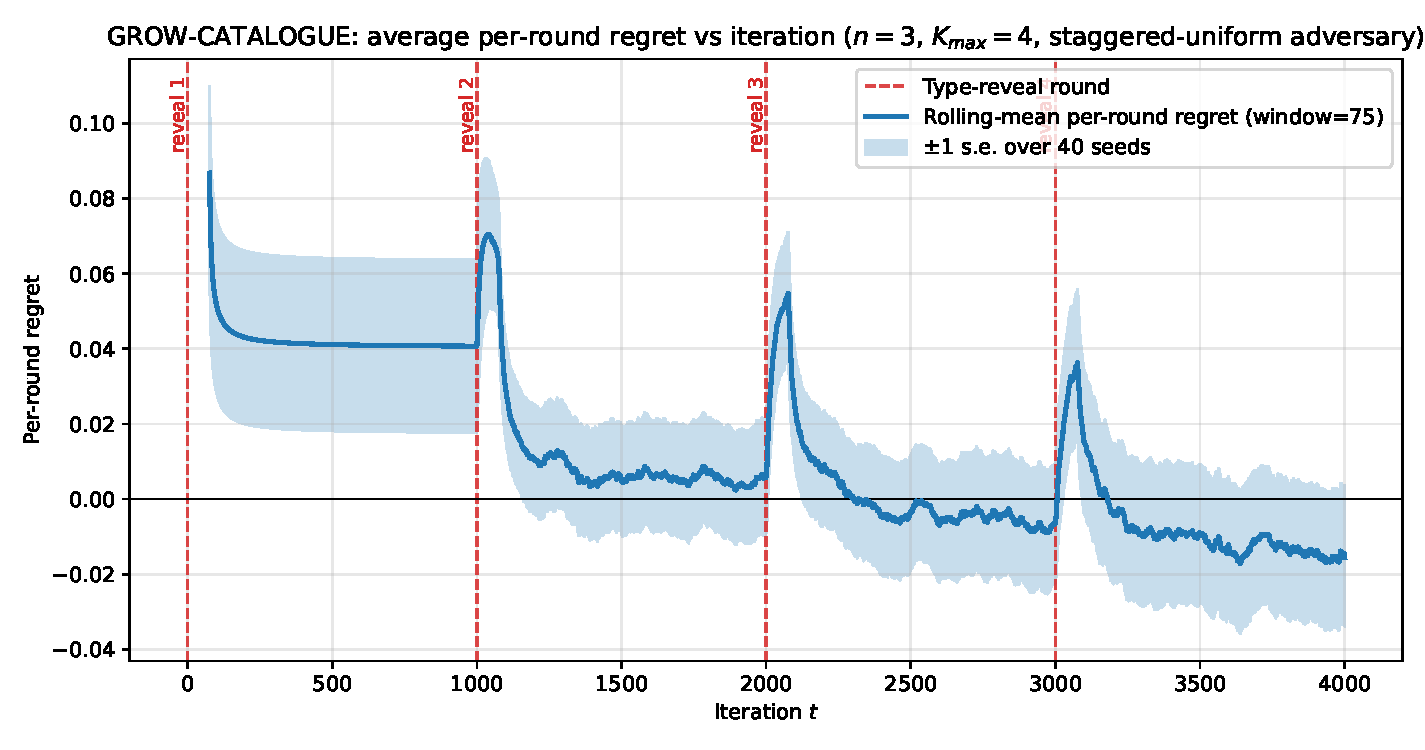
\includegraphics[width=0.98\linewidth]{figures/presentation/avg_regret_per_iter.pdf}
\vspace{-0.5em}
\caption{Rolling-window average per-round regret (window $=75$) for
\textsc{Grow-Catalogue} under the staggered-uniform adversary, averaged
over $40$ random instances. Red dashed lines mark the four discovery rounds
$\tau_i\in\{0,1000,2000,3000\}$. Each reveal causes a visible spike,
followed by re-convergence of the Polynomial-Weights sub-routine within the
new epoch.}
\label{fig:per-round}
\end{figure}

\begin{figure}[t]
\centering
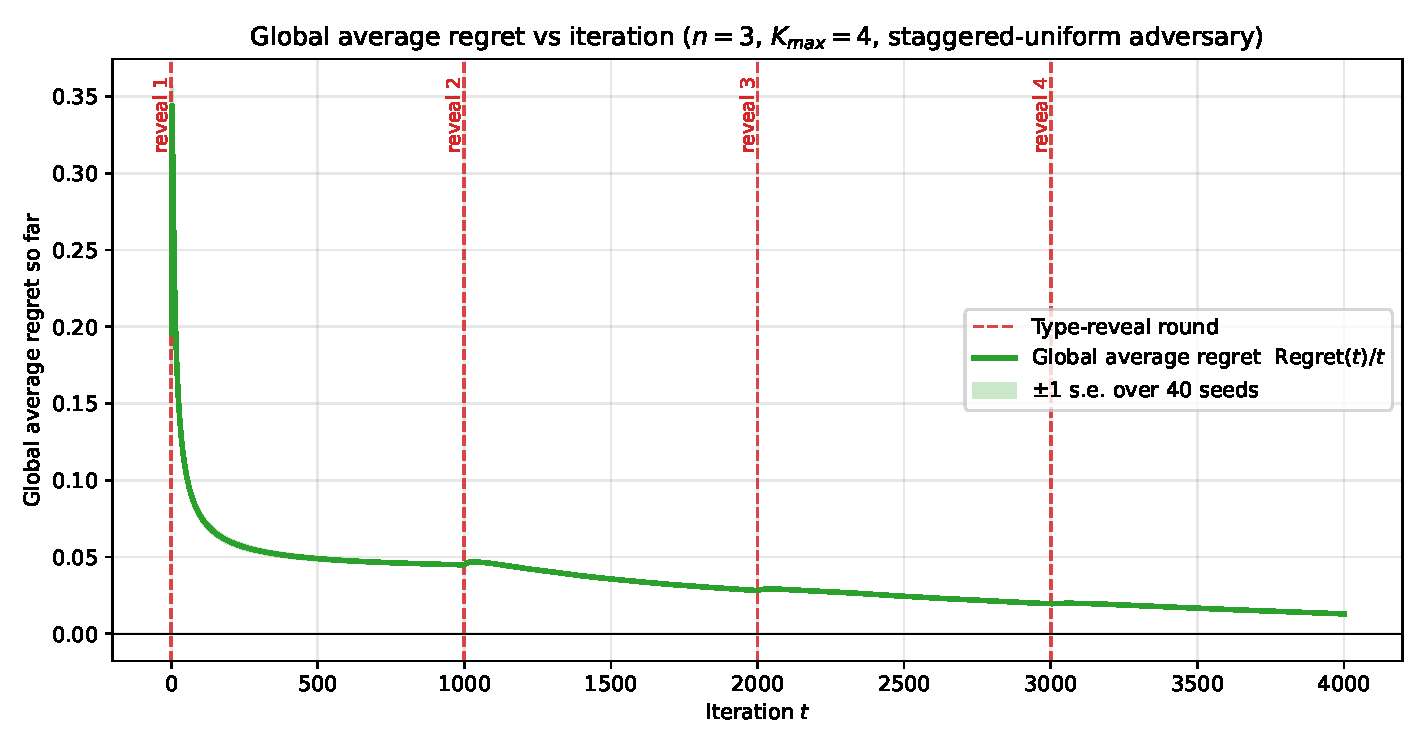
\includegraphics[width=0.98\linewidth]{figures/presentation/global_avg_regret.pdf}
\vspace{-0.5em}
\caption{Global average regret $\mathrm{Regret}(t)/t$ for the same
experiment. The curve tends to $0$ from above, consistent with the
$\tilde O(n\sqrt{\Kmax T})$ upper bound of \Cref{thm:main}. Small bumps at
the discovery rounds confirm the epoch decomposition exploited in the proof.}
\label{fig:global}
\end{figure}

\Cref{fig:per-round} plots the rolling-average per-round regret of
\textsc{Grow-Catalogue}. Two qualitative features of the theorem are
visible. First, at each discovery round $\tau_i$ the per-round regret
\emph{spikes}: the sub-routine has just been handed a new expert set and
must re-learn on it, consistent with the $c_1\sqrt{L_i\log|\cE_i|}$ term
being contributed to the sum by the new epoch. Second, the spike magnitude
\emph{decreases} over successive discoveries, reflecting the fact that
later epochs have larger initial mass at good extreme points inherited
from earlier epochs, and therefore a smaller transient.

\Cref{fig:global} plots the global average regret $\mathrm{Regret}(t)/t$.
It decays rapidly after the first epoch and continues to approach $0$,
empirically confirming the sublinear upper bound. The bumps at $t\in\{1000,
2000,3000\}$ are the same spikes of \Cref{fig:per-round}, averaged into
the global sum.

\Cref{tab:comparison} summarizes the final regret of the four algorithms
evaluated. \textsc{Grow-Catalogue} attains cumulative regret comparable to
the known-$K$ oracle, within $10\%$--$20\%$, and about an order of
magnitude better than the uniform baseline. The total and incremental
variants produce the same regret up to Monte-Carlo fluctuation.

\begin{table}[h]
\centering
\footnotesize
\renewcommand{\arraystretch}{1.15}
\begin{tabular}{lcc}
\toprule
Algorithm & $\EE[\text{Regret}(T)]$ & Ratio\\
\midrule
Known-$K$ oracle         & $14.51\pm 5.00$  & $1.00$\\
\textsc{Grow-Cat.} (total) & $16.57\pm 5.40$  & $1.14$\\
\textsc{Grow-Cat.} (incr.) & $20.26\pm 7.94$ & $1.40$\\
Uniform baseline                & $292.77\pm 350.28$ & $20.18$\\
\bottomrule
\end{tabular}
\caption{Mean $\pm$ std.\ (over 15 seeds) of cumulative regret at $T{=}4000$,
$n{=}3$, $\Kmax{=}3$, uniform-random adversary. The \emph{Known-$K$ oracle}
is \citet[Thm.\,5.1]{balcan2015} run with full knowledge of $K$ from round
$1$; \textsc{Grow-Catalogue} (both variants) attains comparable regret
without this information.}
\label{tab:comparison}
\end{table}

% =============================================================================
\section{Conclusion}
\label{sec:conc}

We gave the first no-regret guarantee for repeated Stackelberg security
games in which the set of attacker types is unknown to the defender in
advance but is assumed to be bounded in size. The \textsc{Grow-Catalogue}
algorithm achieves expected regret
$O\!\bigl(\sqrt{T\Kmax(n^2+\Kmax\log n)}\bigr)$, matching the known-$K$
bound of \citet{balcan2015} with $k$ replaced by the known bound $\Kmax$.
The bound is tight up to logarithmic factors for $\Kmax=O(1)$, gracefully
adapts to the number of types actually observed, and is sublinear in $T$
throughout the useful regime
$\Kmax\cdot(n^2+\Kmax\log n)=o(T)$.

\paragraph{Open problems.}
Three directions for future work stand out. (i) \emph{Partial-information
feedback.} The bandit version of our problem requires a barycentric-spanner
construction whose dimension grows with the catalogue, analogous to
\citet[\S6]{balcan2015}. (ii) \emph{Adaptive adversary.} Our full-
information bound inherits robustness to an adaptive adversary from the
base Hedge analysis, but the partial-information adaptive case is an
explicit open problem in \citet{balcan2015}. (iii) \emph{Shaving log
factors in $\Kmax$.} The sum of per-epoch regrets currently uses a
Cauchy--Schwarz step that loses a $\sqrt{\Kmax}$ factor; sleeping-experts
machinery \citep{mourtada2017} may tighten this to $\sqrt{K'}$ depending
on the actual realized $K'$.

\paragraph{Reproducibility.}
Our Python implementation (NumPy, SciPy, Matplotlib) of
\textsc{Grow-Catalogue}, the baselines, and the experiment harness is
available at
\textcolor{blue}{\href{https://github.com/CS6002-SSG/grow-catalogue}{github.com/CS6002-SSG/grow-catalogue}}.
All experiments in \Cref{sec:exp} can be reproduced by running
\texttt{python plot\_presentation.py} after installing the dependencies
listed in \texttt{requirements.txt}.

% =============================================================================
\bibliography{refs}

\onecolumn
\appendix
% =============================================================================
\section{Implementation Notes}
\label{app:impl}

The main text already contains the full proof of \Cref{thm:main}. This
appendix only collects low-level implementation details of
\Cref{alg:gc}, provided for reproducibility.

\paragraph{Computing $\cE(C;\epsilon)$ in low dimension.}
For $n\le 4$ we enumerate all $(n-1)$-subsets of the hyperplanes that define
the partition of $\cP$ induced by the catalogue, solve the resulting linear
system, and keep each intersection point that lies in $\cP$. The set of
hyperplanes consists of (i) $n$ simplex constraints ($p_i\ge 0$ and the
bounding hyperplane of $\cP$), and (ii) $|C|\binom{n}{2}$ pairwise
best-response constraints, one per pair of targets per attacker type. For
$n=3$, $\Kmax=4$ this gives at most $4+4\cdot 3=16$ hyperplanes and
$\binom{16}{2}=120$ candidate intersections, which is tractable.

\paragraph{Anytime learning rate.}
The learning rate $\eta_t=\sqrt{\log|\cE|/t}$ is a standard anytime
schedule \citep[e.g.,][Ch.~2]{cesa2006} that avoids needing to know the
epoch length $L_i$ in advance. It guarantees the $\sqrt{L_i\log|\cE|}$
regret bound of \Cref{prop:hedge} without any horizon parameter, which
is what allows Step~3 of the proof to go through after every restart.

\paragraph{Total vs.\ incremental recomputation.}
The total variant rebuilds $\cE(C;\epsilon)$ from scratch on every
discovery round; the incremental variant keeps all old vertices that
still lie on the boundary of some region after the refinement and only
computes new vertices at intersections of old region boundaries with the
new hyperplanes introduced by the discovered type. Both produce the same
$\cE(C;\epsilon)$ and hence the same per-step distribution, which is why
the two variants are statistically indistinguishable in
\Cref{tab:comparison}.

\paragraph{Hyperparameters in the experiments.}
The staggered-uniform adversary uses horizon $T=4000$ split into
$\Kmax=4$ phases of $1000$ rounds. The rolling window for
\Cref{fig:per-round} is $75$ rounds. Each configuration is averaged over
$40$ random game instances.
Dependencies: \texttt{numpy>=1.26}, \texttt{scipy>=1.11},
\texttt{matplotlib>=3.8}. The full code and a \texttt{requirements.txt}
are in the GitHub repository linked in \Cref{sec:conc}.


\end{document}
